\section{Proposed deep learning architecture}
\paragraph{}
In this section, we present the \ac{dl} architecture used for \ac{slr} using the TAKALEM Gloves. The architecture consists of an input layer, an \ac{lstm} layer, and an output layer, and it is designed for both words and characters classification.
\paragraph{}
Input Layer: The input layer receives the sensor data collected from the TAKALEM Gloves. The dataset is reshaped to have a shape of (3360, 150, 11), where 3360 represents the number of gestures used for training, 150 represents the number of rows for each gesture, and 11 represents the number of features. The features include the flex sensor readings, gyro data, and raw acceleration values.
\paragraph{}
\ac{lstm} Layer: The \ac{lstm} layer is a crucial component of the architecture as it captures the sequential information and temporal dependencies present in the \ac{sl} gestures. It is responsible for learning the patterns and dynamics of hand movements and finger positions. The \ac{lstm} layer processes the input sequence and retains information over extended time periods, mitigating the vanishing gradient problem. In our model we used 38 nodes for this layer, we tried different number of nodes, and we noticed that the accuracy is getting higher as the number of nodes is getting higher, but we chosen exactly 38 because it's the highest possible number that the esp32 can handle duo to it's limits of flash memory.
\paragraph{}
Output Layer: The output layer is the final layer of the architecture and is responsible for generating predictions. For the words classification model, the output layer has 14 nodes, representing the 14 different words in the dataset. For the characters classification model, the output layer has 26 nodes, representing the 26 letters of the alphabet. The output layer applies a \textit{softmax} activation function to produce a probability distribution over the classes, with the highest probability indicating the predicted sign.
\paragraph{}
The proposed architecture is trained using the reshaped dataset, with appropriate training, validation, and testing splits. The model's parameters are adjusted during the training process using Adam as optimization algorithm, and "categorical cross-entropy" is chosen for loss function.
\paragraph{}
The performance of the architecture is evaluated using various evaluation metrics, including accuracy, precision, recall. These metrics assess the model's ability to correctly classify \ac{sl} gestures and provide insights into its overall effectiveness.
\paragraph{}
The architecture is implemented using TensorFlow python library, which provide efficient tools for constructing and training \ac{ann}s like \ac{lstm}. The training process can benefit from powerful computing resources, such as GPUs, to accelerate the training time and handle the large-scale nature of the dataset .
\paragraph{}
By utilizing the proposed deep learning architecture in figure \ref{fig:model}, the TAKALEM Gloves demonstrate promising results in \ac{slr}. The model's ability to accurately classify both words and characters is a significant step towards enabling effective communication for individuals using \ac{sl}.
\begin{figure}[h]
	\centering
	\begin{subfigure}[b]{0.2\textwidth}
		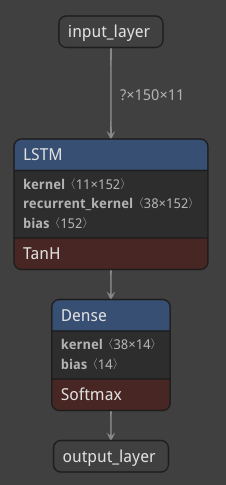
\includegraphics[width=\textwidth]{images/model_words}
		\caption{Words model}
		\label{fig:words_model}
	\end{subfigure}
	\begin{subfigure}[b]{0.2\textwidth}
		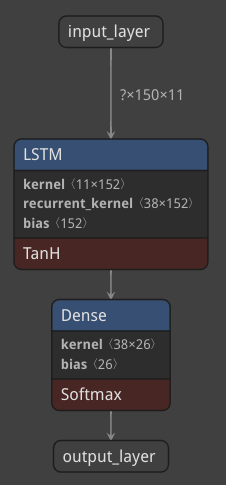
\includegraphics[width=\linewidth]{images/model_characters}
		\caption{Characters model}
		\label{fig:characters_model}
	\end{subfigure}
	\caption{The trained model}
	\label{fig:model}
\end{figure}
\paragraph{}
In order to be able to use the model on the esp32, we should convert it to tensorflow lite version, and then convert it to a c++ array, as shown in figure \ref{fig:model_tf}, the tflite use different naming for different layers, the \textbf{\ac{lstm}} layer become \textbf{UnidirectionalSequenceLSTM}, and the \textbf{Dense} layer become \textbf{FullyConnected}. The size of the c++ array for the model is 37452 for characters model, and 35580 for words model.
\begin{figure}[h]
	\centering
	\begin{subfigure}[b]{0.2\textwidth}
		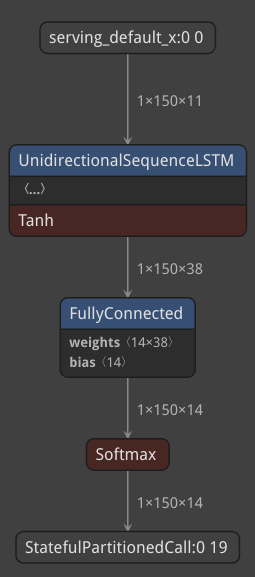
\includegraphics[width=\textwidth]{images/tf_model_words}
		\caption{Words model}
		\label{fig:words_model_tf}
	\end{subfigure}
	\begin{subfigure}[b]{0.2\textwidth}
		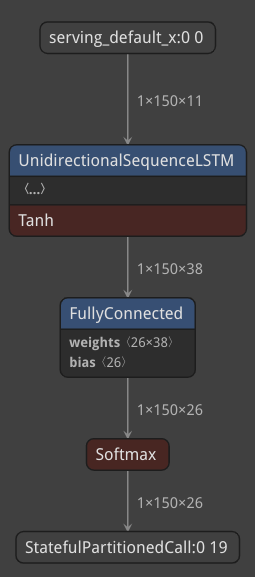
\includegraphics[width=\linewidth]{images/tf_model_characters}
		\caption{Characters model}
		\label{fig:characters_model_tf}
	\end{subfigure}
	\caption{The trained model after converted to tflite model}
	\label{fig:model_tf}
\end{figure}
